\documentclass[12pt]{article}
\usepackage{graphicx} % Required for inserting images
\usepackage{titling} % For custom title page
\usepackage{url}
\renewcommand{\familydefault}{\sfdefault}
\usepackage{parskip} % For spacing between paragraphs

\title{Analysing the Effectiveness of Consumer-ready Simulation Software in Training for Maritime Navigation Under Pressure}
\author{Richard Lay-Flurrie}
\date{\today}

\pretitle{
  \begin{center}
  
\includegraphics[width=0.2\textwidth]{images/logo.jpeg}\vspace{2em} \\
  \LARGE
}
\posttitle{
  \end{center}
}

\begin{document}

\maketitle
\thispagestyle{empty}

\begin{center}
  \vfill
  \large
  A thesis submitted for the degree of\\
  Doctor of Philosophy\\
  \vfill
  \normalsize
  School of Computer Science and Electronic Engineering\\
  University of Essex\\
  \vfill
\end{center}

\newpage

\section*{Acknowledgements}

Lorem ipsum dolor sit amet, consectetur adipiscing elit, sed do eiusmod tempor incididunt ut labore et dolore magna aliqua. Ut enim ad minim veniam, quis nostrud exercitation ullamco laboris nisi ut aliquip ex ea commodo consequat. Duis aute irure dolor in reprehenderit in voluptate velit esse cillum dolore eu fugiat nulla pariatur. Excepteur sint occaecat cupidatat non proident, sunt in culpa qui officia deserunt mollit anim id est laborum.

Lorem ipsum dolor sit amet, consectetur adipiscing elit, sed do eiusmod tempor incididunt ut labore et dolore magna aliqua. Ut enim ad minim veniam, quis nostrud exercitation ullamco laboris nisi ut aliquip ex ea commodo consequat. Duis aute irure dolor in reprehenderit in voluptate velit esse cillum dolore eu fugiat nulla pariatur. Excepteur sint occaecat cupidatat non proident, sunt in culpa qui officia deserunt mollit anim id est laborum.

\newpage

\section*{Abstract}

Lorem ipsum dolor sit amet, consectetur adipiscing elit, sed do eiusmod tempor incididunt ut labore et dolore magna aliqua. Ut enim ad minim veniam, quis nostrud exercitation ullamco laboris nisi ut aliquip ex ea commodo consequat. Duis aute irure dolor in reprehenderit in voluptate velit esse cillum dolore eu fugiat nulla pariatur. Excepteur sint occaecat cupidatat non proident, sunt in culpa qui officia deserunt mollit anim id est laborum.

Lorem ipsum dolor sit amet, consectetur adipiscing elit, sed do eiusmod tempor incididunt ut labore et dolore magna aliqua. Ut enim ad minim veniam, quis nostrud exercitation ullamco laboris nisi ut aliquip ex ea commodo consequat. Duis aute irure dolor in reprehenderit in voluptate velit esse cillum dolore eu fugiat nulla pariatur. Excepteur sint occaecat cupidatat non proident, sunt in culpa qui officia deserunt mollit anim id est laborum.

Lorem ipsum dolor sit amet, consectetur adipiscing elit, sed do eiusmod tempor incididunt ut labore et dolore magna aliqua. Ut enim ad minim veniam, quis nostrud exercitation ullamco laboris nisi ut aliquip ex ea commodo consequat. Duis aute irure dolor in reprehenderit in voluptate velit esse cillum dolore eu fugiat nulla pariatur. Excepteur sint occaecat cupidatat non proident, sunt in culpa qui officia deserunt mollit anim id est laborum.

Lorem ipsum dolor sit amet, consectetur adipiscing elit, sed do eiusmod tempor incididunt ut labore et dolore magna aliqua. Ut enim ad minim veniam, quis nostrud exercitation ullamco laboris nisi ut aliquip ex ea commodo consequat. Duis aute irure dolor in reprehenderit in voluptate velit esse cillum dolore eu fugiat nulla pariatur. Excepteur sint occaecat cupidatat non proident, sunt in culpa qui officia deserunt mollit anim id est laborum.

\newpage

\tableofcontents

\newpage

\listoftables

\newpage

\listoffigures

\section{Introduction}

\subsection{Research Questions}

What measurable physiological indicators correlate with preceived stress during challenging simulation tasks?

What is the impact of exposure, at different levels, to high-pressure scenarios in a virtual environment on a person's ability to make decisions in real life?

How do decision stressors impact the performance of users undertaking maritime navigation tasks in a virtual environment?

How do stress levels of volunteers in simulated high-pressure maritime navigation situations compare to volunteers in real maritime navigation?

Is there a difference in performance of volunteers in high-pressure maritime navigation situations in virtual worlds as compared to the real world?

\subsection{The Benefits of Consumer-ready Simulation in Training}

Simulation is a powerful tool for training, especially for high-pressure scenarios. It allows people to practice skills in a controlled environment without the risk of injury or damage to overly expensive equipment. With the cost of a consumer-ready simulator setup being under £1,000, it can be a cost-effective way of training for a multitude of scenarios.


\subsection{Consumer-ready Simulation Software}

Consumer/customer ready products are ones which are "fully functioning and ready for shipment to and use by an end user which does not require manufacturing or integration services". \cite{LawInsiderCustomerReady} In the context of simulation software, this means that the software is "plug and play", such as a video game, requiring minimal technical knowledge to operate. 

While being "plug and play" is also possible with commercial simulation software, it is also often very expensive \cite{ESIGamesStore}\cite{BISimVBS4Update} or only available to certain industries, due to it containing trade or military secrets \cite{BISimShipWalkthrough}. 


\subsubsection{Sectors}

Many sectors such as military, search and rescue, farming, factory work, driving and aviation have consumer-ready simulation software available. These are widely used for recreation purposes but can also be used for training. For example, the game Stormworks: Build and Rescue \cite{stormworks} allows players to build and operate their own search and rescue vehicles in a variety of realistic scenarios. The Arma series allows players to create and play out military scenarios in realistic environments \cite{arma3} with groups of people often meeting up online on a regular basis to play these scenarios for enjoyment \cite{42CommandoArma3} \cite{BourboneFreeman}. These military simulation communities are able to achieve impressive levels of realism in their scenarios, often with little to no real life military experience of their own. 

\subsubsection{Building Virtual Environments}

Many types of simulation software are released with some form of tools which allow users to create their own virtual environments.

\subsubsection{Using Ready Made Virtual Environments}

\subsection{The Importance of Training for High-pressure Scenarios}

\subsection{Maritime Navigation Under Pressure} 

\section{Literature Review}

\subsection{Maritime Navigation Training}

In maritime navigation, the study of certain instruments and other sources of information is often required. Charts, dividers, overlays, menus, ship information, tasks lists and detailed task information may all need to be studied. \cite{atik2019use} The simulation of these instruments and sources of information in virtual environments can be achieved as seen in commercial software such as the game Stormworks: Build and Rescue \cite{stormworks} and Arma 3 \cite{arma3} (see Figure \ref{fig:tamarclassstormworks}) (see Figure \ref{fig:falklandsarma}).

\begin{figure}[h]
  \centering
  \begin{minipage}[b]{0.9\linewidth}
    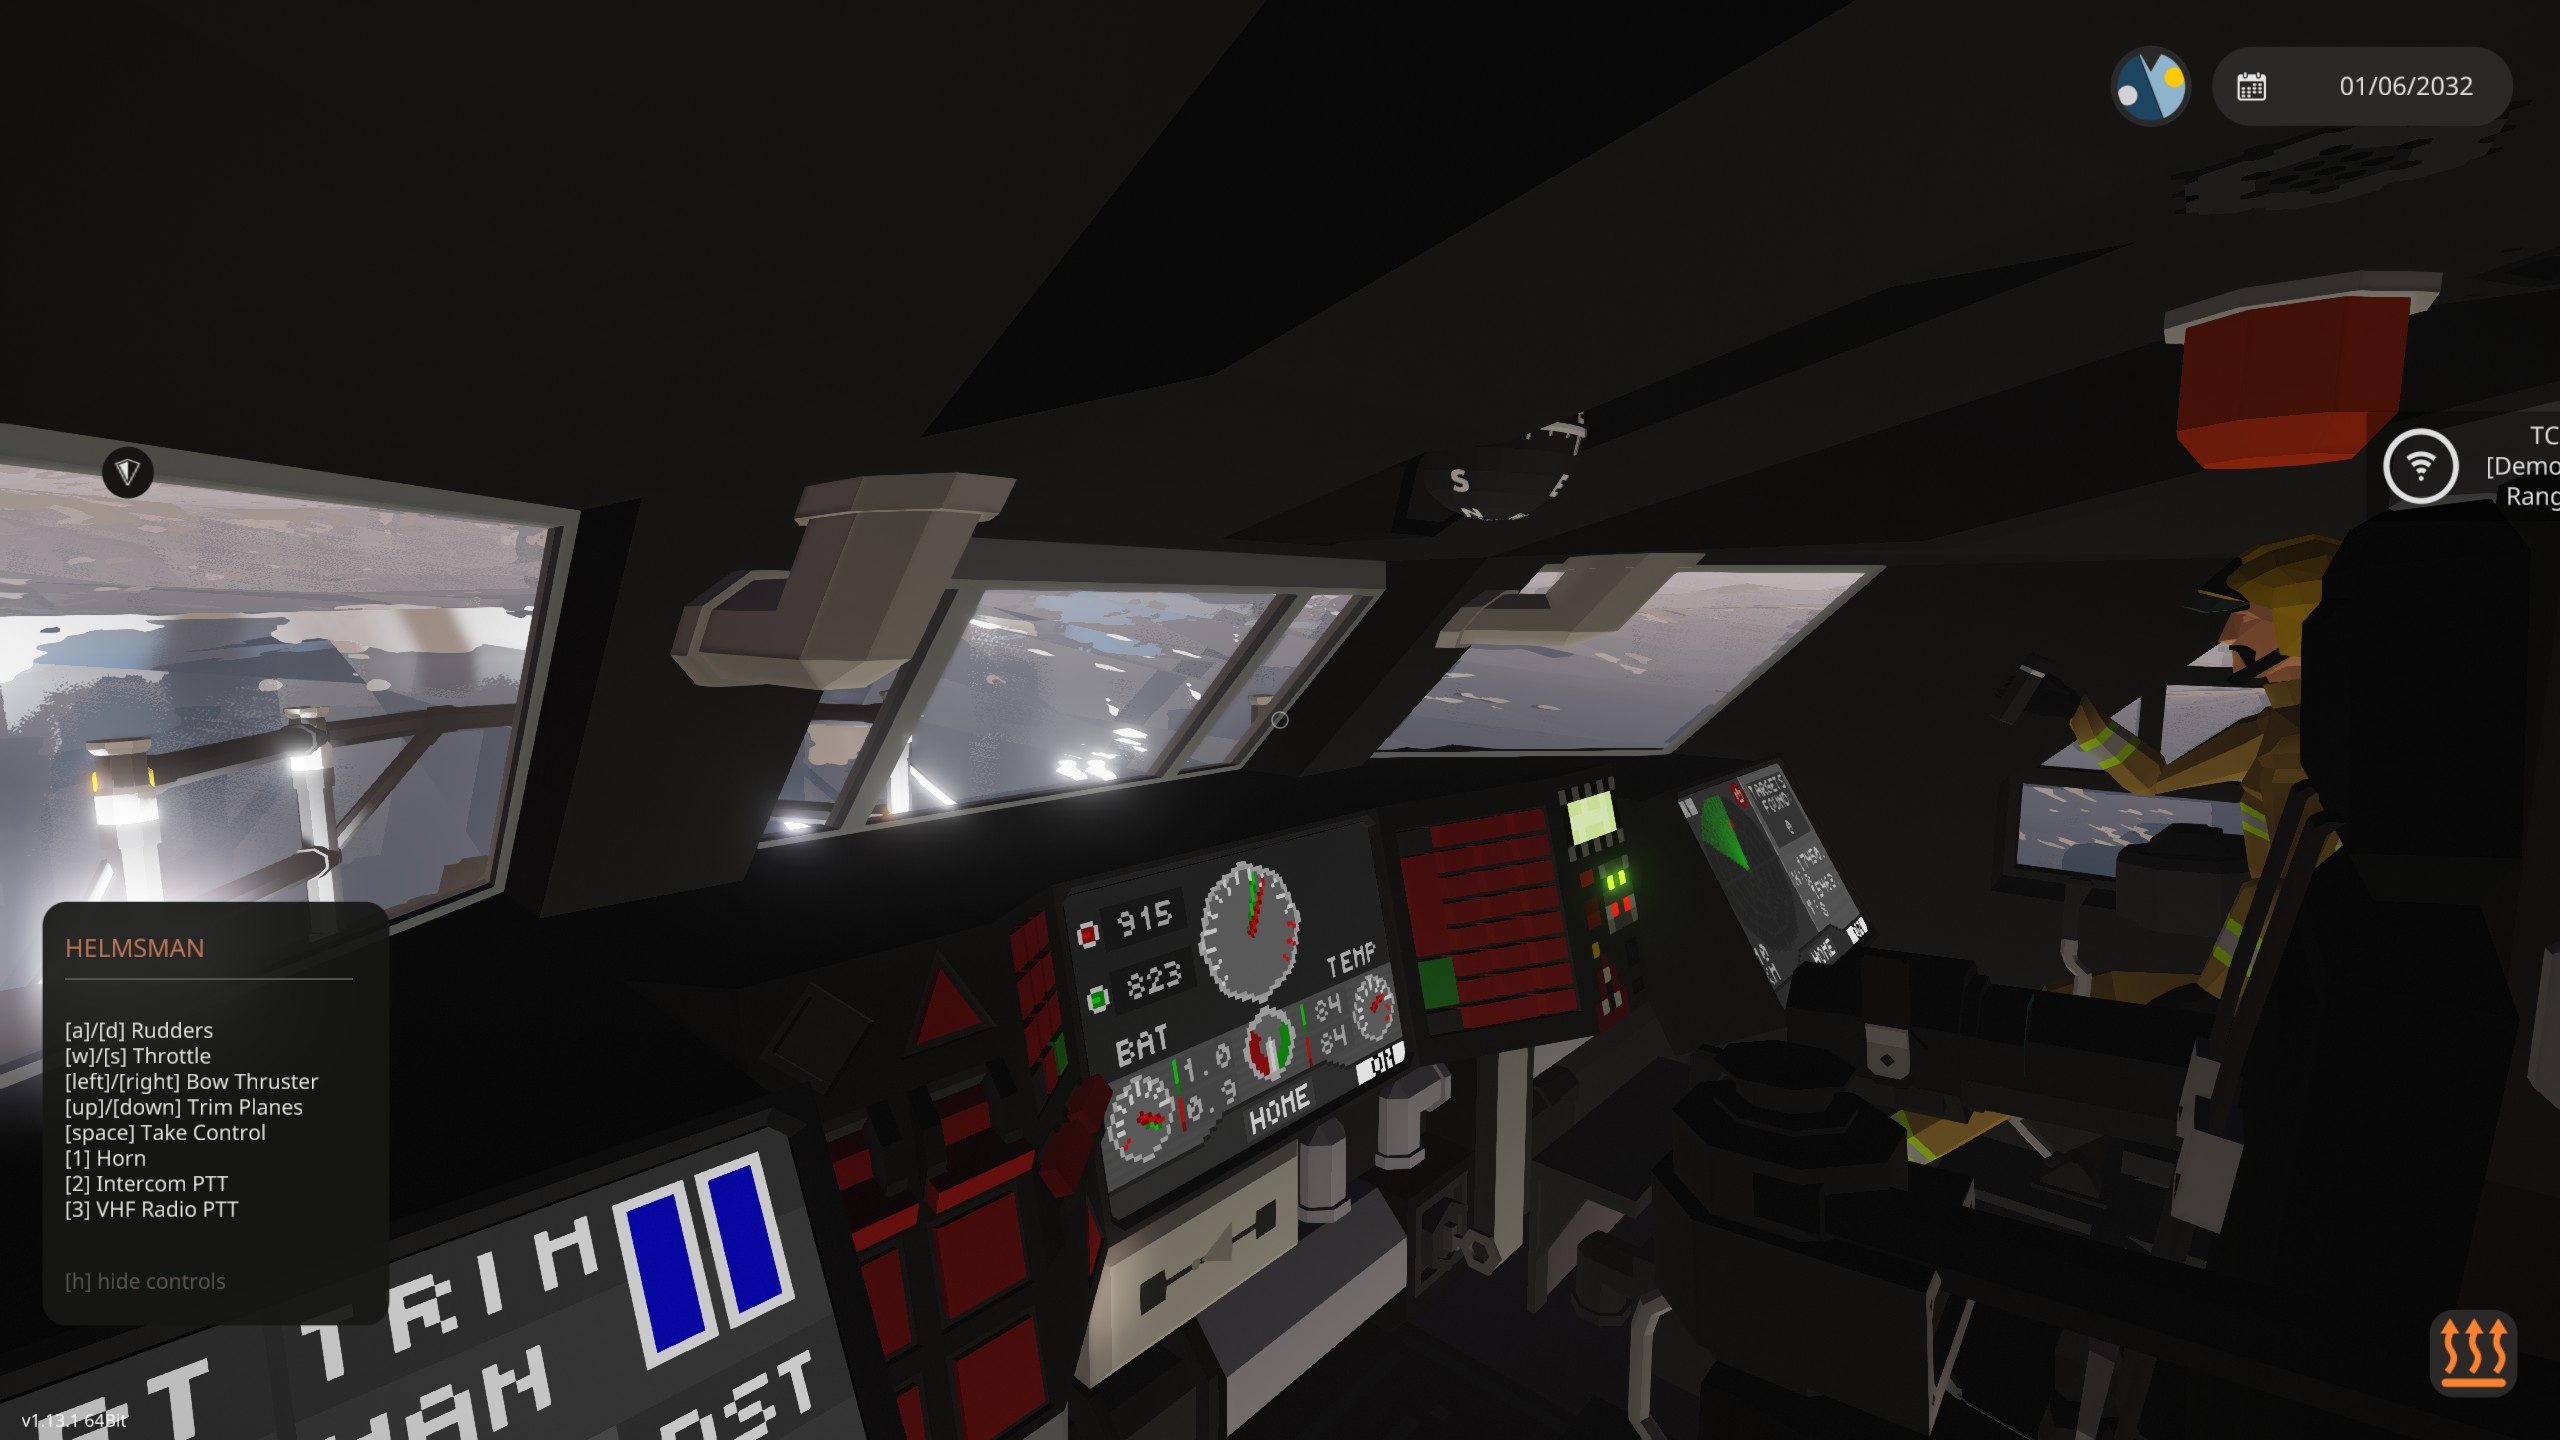
\includegraphics[width=\linewidth]{images/tamar-class-lifeboat-stormworks.jpg}
    \caption{Digital twin of a Tamar Class Lifeboat in Stormworks: Build and Rescue}
    \label{fig:tamarclassstormworks}
  \end{minipage}
\end{figure}

\begin{figure}[h]
  \centering
  \begin{minipage}[b]{0.9\linewidth}
    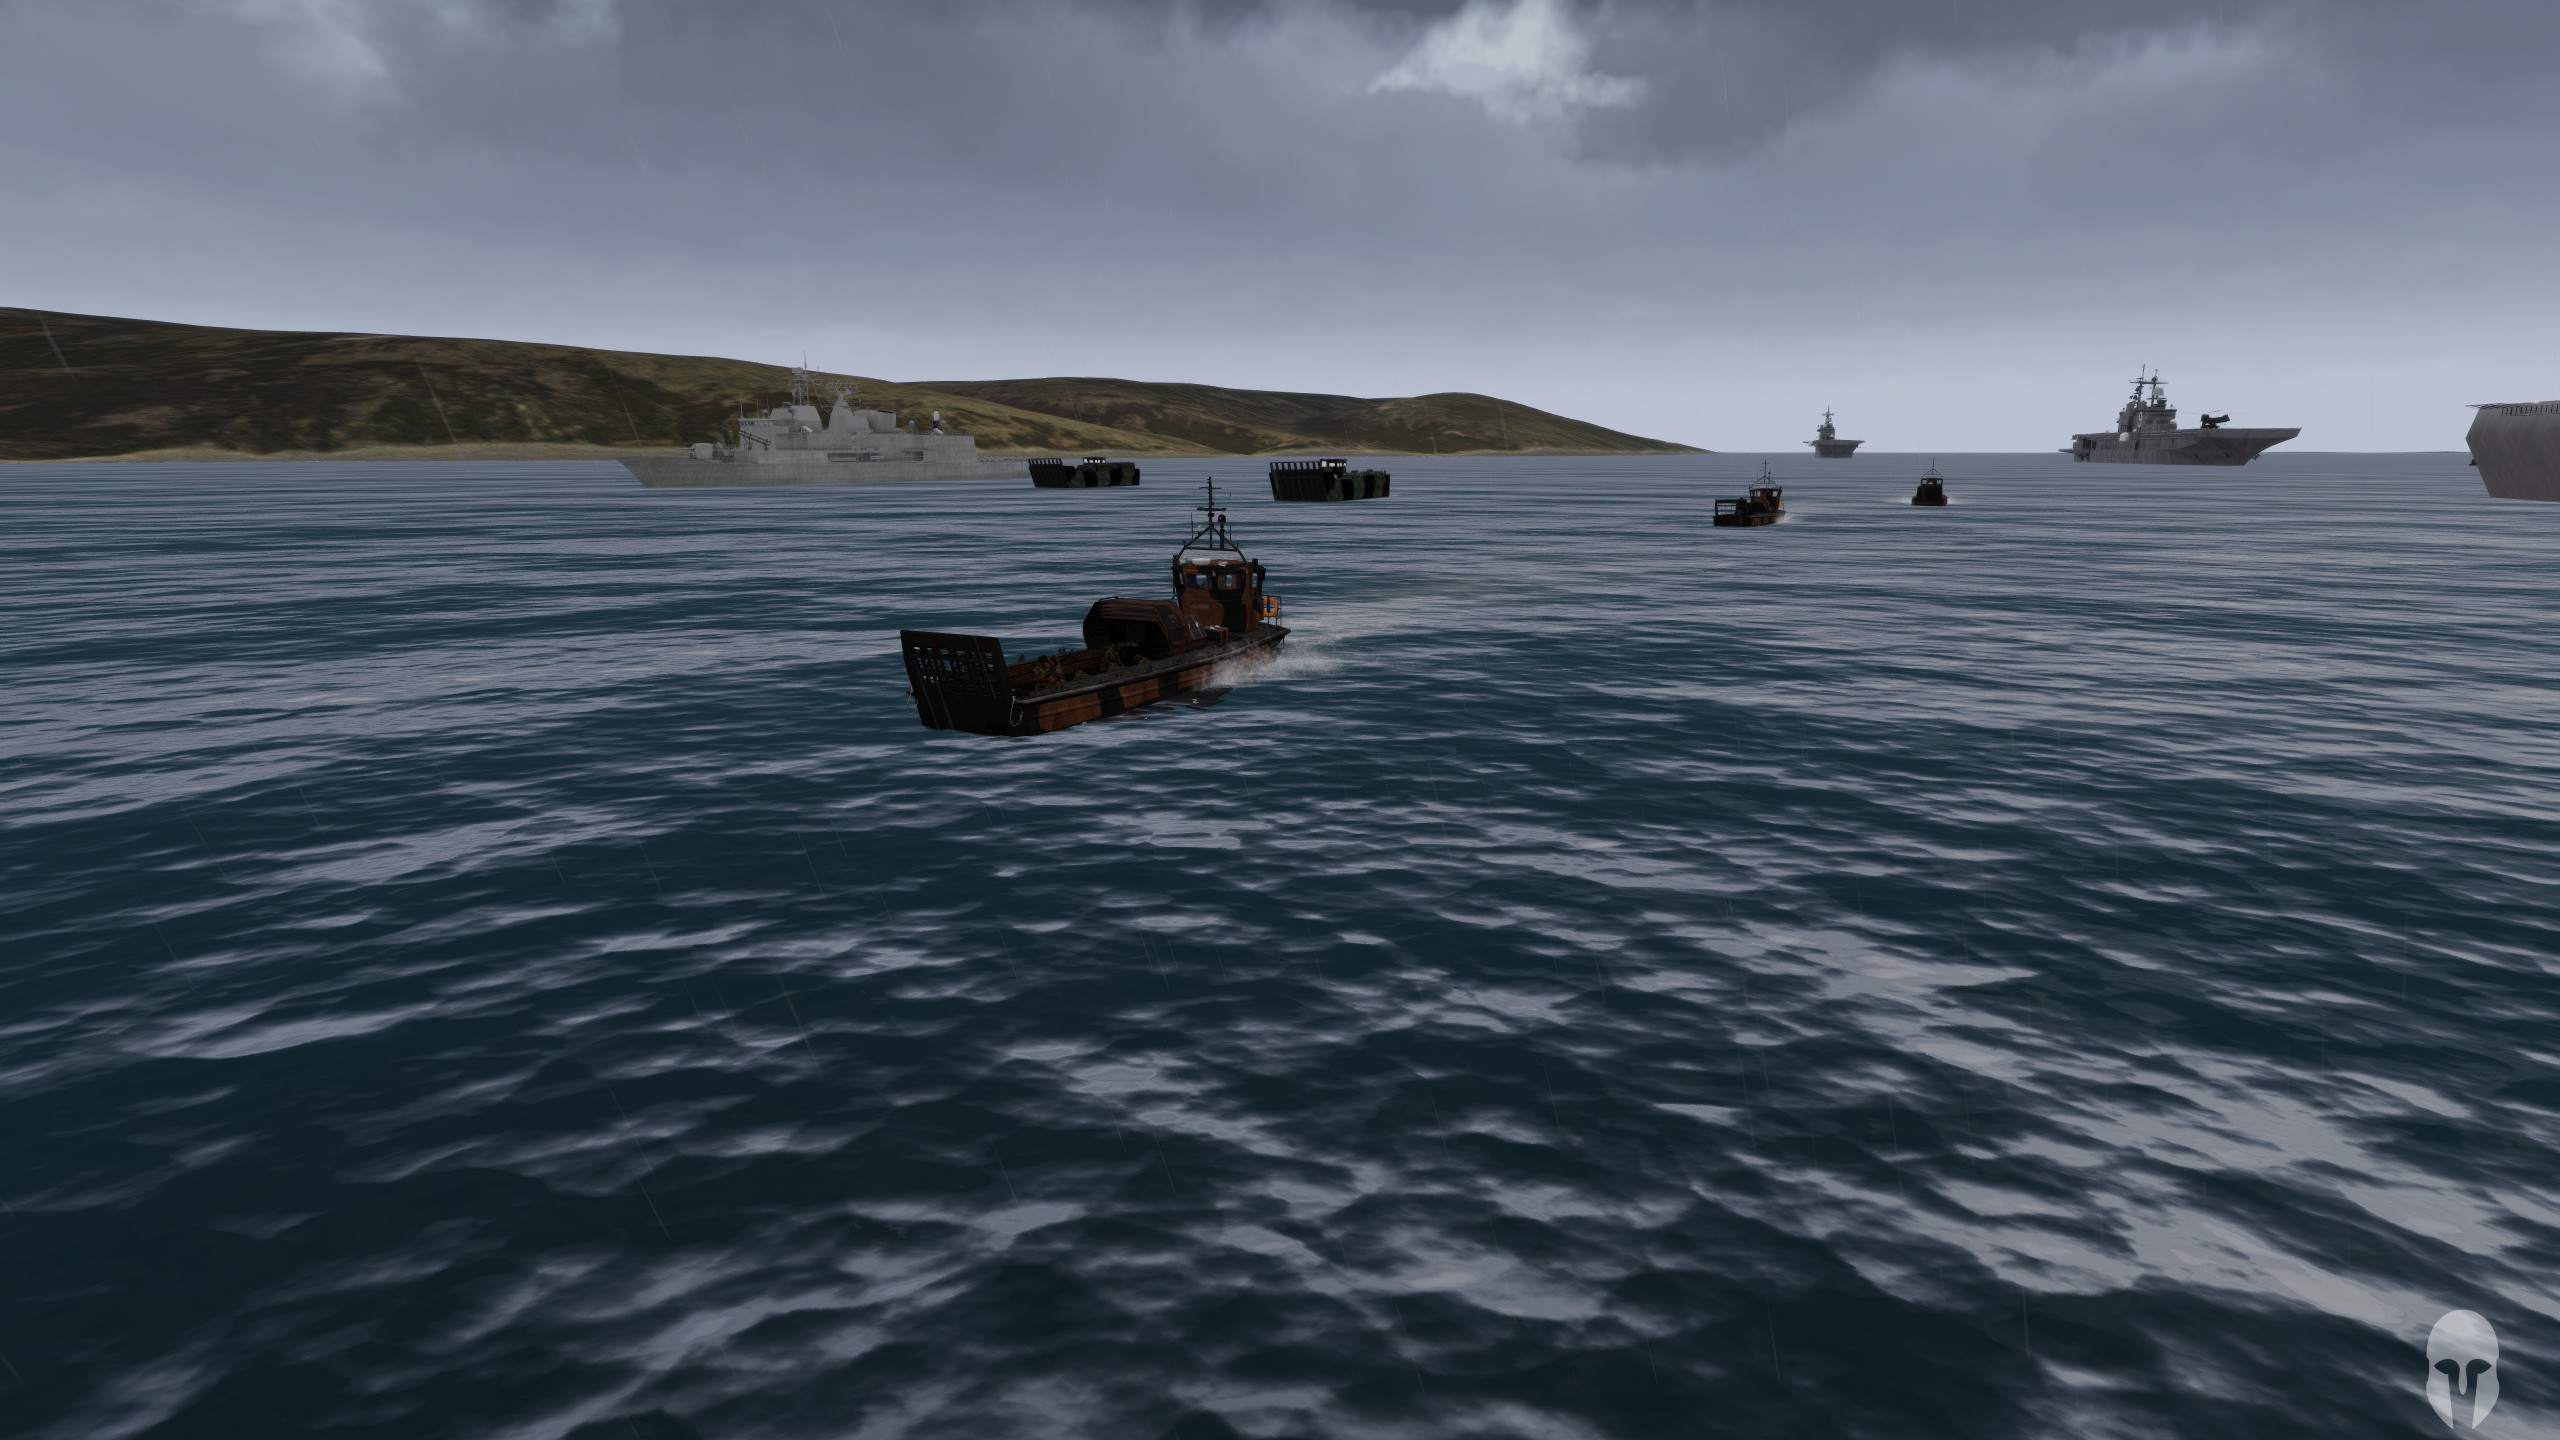
\includegraphics[width=\linewidth]{images/falklands-arma.jpg}
    \caption{Simulated Falklands War scenario in Arma 3}
    \label{fig:falklandsarma}
  \end{minipage}
\end{figure}

\subsection{High-pressure Scenarios and Decision-making}

A high-pressure situation is one which can be defined as a scenario where an invidual has a difficult task or decision to make, which is likely to make the individual feel stressed or anxious. In such situations, the individual may experience a range of physiological and psychological responses, such as increased heart rate, sweating, and impaired cognitive function. These responses can impact the individual's ability to think clearly and make effective decisions, which can have serious consequences in critical situations.

Some examples of high-pressure situations include emergencies, meeting deadlines, public speaking and competitive activities. They do not necessarily have to be life-threatening or pose a great risk to the individual to be considered high-pressure. One such example in popular media is Richie's Plank Experience \cite{richiesplank}, a virtual reality game in which the player has to walk across a plank suspended high above the ground. Although the player is not in any real danger, the immersive nature of the virtual reality experience can trigger a fear response, making it a high-pressure scenario. \cite{el2023walk}

Some factors which can contribute to the experience of stress in a situation are information overload, time pressure, complexity and uncertainty. \cite{Phillips-Wren18082020} Fear can also be considered a factor which contributes to the experience of stress. \cite{klein2013effect} Fear results from the perception of threat of danger to the person and can greatly impact decision making abilities by causing a person to focus only on things which they deem to be "catastrophic" in a given scenario. \cite{chanel2009influence} For example, in a survival situation, one may be so focused on avoiding a threat that they struggle to open a door.

\subsection{Necessity for Regular Exposure to High-pressure Scenarios}

Certain career paths require individuals to regularly make decisions under pressure such as emergency service \cite{gullon2024prevalence}\cite{smith2011work}, military \cite{srivastava2023occupational}\cite{hellewell2018measuring}\cite{fear2009job} and transport \cite{jiao2023physiological}\cite{cahill2021pilot} personnel. In these professions, the ability to think clearly and make sound decisions under pressure is critical to the safety and well-being of the individual and other people they may come in contact with or be responsible for, either directly or indirectly \cite{mcfarlane2021investigating}. 

For example, armed police officers may be required to make a decision on whether or not to deploy lethal force in a situation which is influenced by all of the aforementioned decision stressors, including fear. For many people, this is a scenario which they are unlikely to ever have to face. However, armed police officers could, in theory, have to make this decision regularly. 

\subsection{Training for High-pressure Scenarios}

Repeat exposure to the feeling of stress can help individuals to become more accustomed to it and learn how to deal with it. For this reason, military training around the world is normally designed to be stressful and, at times, unplesant. 

One such example of this is the shouting and aggression which is often used by instructors to help recruits become accustomed to thinking while under the stress of noise and unplesant attention.

As portraited in the film "Jarhead", which is based on the training of United States Marines in the early 1990s, in one scene Jake Gyllenhall's character is being slapped on the back of the head by the senior drill instructor while he is trying to recite some information. The recruit character states that he can't think while being hit on the head and the senior drill instructor retors that if he can't think while being slapped on the head, how does he expect to effectively fire his rifle in combat, an inherently stressful situation \cite{jarhead2005}.

Training for high-pressure scenarios can also take place in virtual environments. Simulations can be designed to invoke the feeling of stress in a controlled environment. A study on pilots from Fire and Emergency New Zealand found that, stress levels experienced in VR training scenarios can be very similar to those experience in the real-life scenarios. \cite{clifford2019creating}

\subsection{Application of Virtual Environments for Training}

Realistic virtual environments are ones which immerse users in a scenario by making it as close to the real thing as possible. Having access to physical objects and the use of one's own body to interact with the environment are preferred methods of immersion. \cite{clifford2018effect}

Realism can be measured both objectivly and subjectively. \cite{gonccalves2022systematic} Objective realism is the extent to which the virtual environment is similar to the real world. Subjective realism is the extent to which the user believes the virtual environment is real. Users can perceive different levels of realism in the same virtual environment. For example, some users may hone in one the graphical fidelity of the environment, while others may focus on the interactive elements such as physics and object manipulation. One study refers to a focus on the look of a virtual environment as the "fidelity trap", as it is not safe to "assume that students learn to the level of realism". \cite{carey2020high}

Realistic virtual environments can be used to effectively convey information to people in a way that is engaging and memorable. As a bonus, access to modern hardware allows for these experiences to be had at home \cite{anderson2024blending} and not require a visit to a dedicated site, which historically was the norm. \cite{Scott2022}

\subsubsection{Success in other Industries}

The use of virtual environments has applications in other industries such as the delivery of laboratory safety training, \cite{makransky2019motivational}, medical training (bone and dental surgery, intubation procedures, eye surgery etc.) \cite{ruthenbeck2015virtual} and welding training \cite{da2010use}. 

\subsection{Virtual Reality (VR)}

Virtual reality is a technology which immerses users in a virtual environment by employing hardware such as goggles, headsets, gloves or body suits to simulate the experience of "being there". This is known as telepresence. \cite{britannicaVR}

Commercially available VR devices, often used for recreation, including devices such as the Oculus series of headsets (Rift S, Quest 2) \cite{greenwald2020} can be used for training purposes. \cite{kaplan2021effects}\cite{axonVRTraining}\cite{axonVRTrainingUK}

"It's a whole new level. You know, your heart rate gets pounding. You feel emotionally invested. You start sweating and you really feel that stress and that realism that you would in that situation"

"I have never seen the sort of intense demand that we're seeing for virtual reality training." - Rick Smith AXON CEO and Founder. \cite{axonYouTube}

\subsubsection{Advandages of VR for Training}

Virtual reality is now widely accessible, with the cost of a used Oculus Rift S headset being less than £100. Paired with a decent gaming computer, the cost of entry to a high fidelity VR simulation is at its lowest ever.

\begin{figure}[h]
  \centering
  \begin{minipage}[b]{0.9\linewidth}
    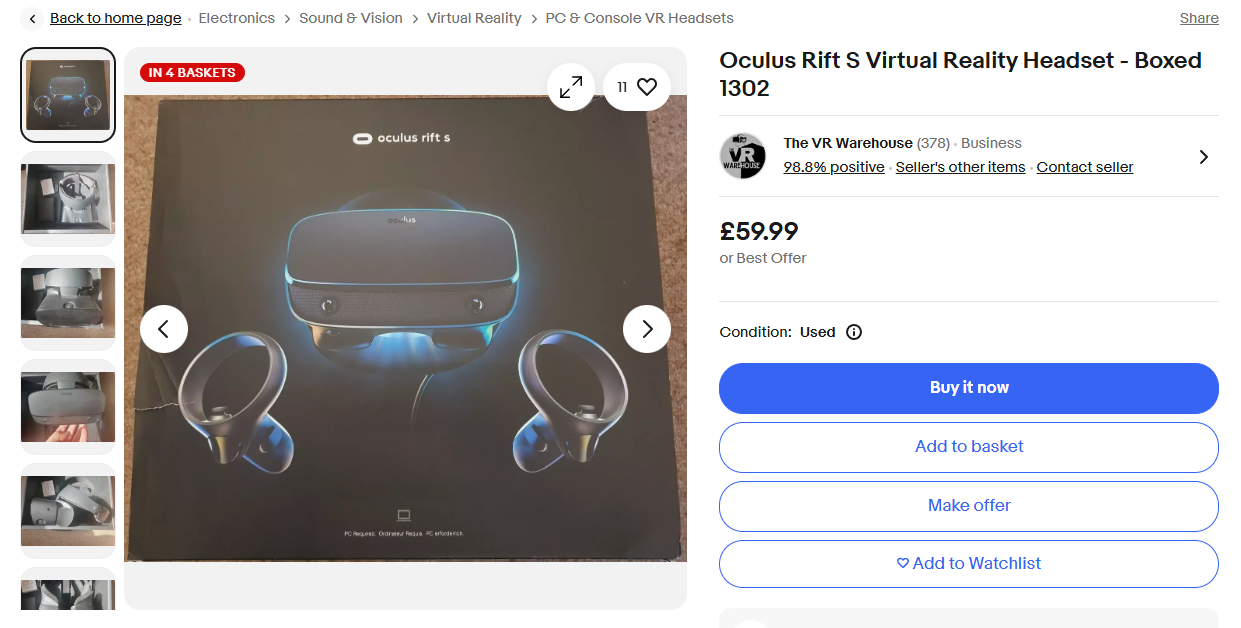
\includegraphics[width=\linewidth]{images/ebay-screenshot-rift-s.png}
    \caption{The cost of a boxed Oculus Rift S headset on Ebay as of 15th March 2025}
    \label{fig:ebayOculusRiftS}
  \end{minipage}
\end{figure}


This is a significant advantage of VR for training as it begins as a cost-effective method of reducing the risk of injury to personnel and damage to equipment. Furthermore, VR training can allow people access to environments, in true to life scale, at the same time as other people, regardless of their location (assuming they have enough space to move around in). This is an advantage over traditional monitor-based immersive environments which don't give the sense of presence that VR does \cite{makransky2017development}.

\subsubsection{Disadvantages of VR for Training}

One main disadvantage of VR is the potential for the user to experience virtual reality sickness (VR sickness). VR sickness can be caused by the user perceiving self-motion by moving around in the virtual environment while remaining stationary in the real world. This can cause the user to feel symptoms which are very similar to motion sickness. \cite{chang2020virtual} This has been a recognised disadvantage of VR since at least 1995 \cite{regan1995investigation}, when the technology was not readily available to the public and is still an on-going issue. While some different games and pieces of hardware attempt to alleviate the symptoms, such as narrowing the field of view while a person is moving in game \cite{RecRoomVRMovement}\cite{fernandes2016combating}, the issue is still present.

Studies of psychological effects of long term exposure to VR

\subsubsection{Digital Twins}

A digital twin is "a virtual representation of an object or system designed to reflect a physical object accurately." \cite{ibmDigitalTwin} Digital twins are commonly found in video games with the primary use being for recreation. Digital twins of real world items are especially prevalent in games which replicate the real world. For example, aircraft and naval assets in Digital Combat Simulator World \cite{dcsworld}, vehicles in the racing simulation iRacing \cite{iracing} or weapons in the first person shooter series Battlefield \cite{battlefield4}. However, digital twins can also be used for training purposes such as in the logistics industry \cite{longo2023prepare} and in the military \cite{ukcatt}.

Digital twins provide a key benefit to training in virtual environments in that they can be used to demonstrate how a physical object or system works and allow a user to experiment with it in a controlled environment. For example, a digital twin of a ship's bridge can be used to train maritime navigation students on how to use the equipment in a safe environment. 

Digital twins do also have limitations in that, if not implemented accurately, they can provide unrealistic expectations of the real thing. During a demonstration of a proposed animatronic doll for a project, Youtuber Michael Reeves demonstrates how the digital twin can rotate its jaw through 360 degrees. (see Figure \ref{fig:michaelreeves}) "Uhh, ooo, can't do that in real life" he says. \cite{reevesYouTube}

\begin{figure}[h]
  \centering
  \begin{minipage}[b]{0.9\linewidth}
    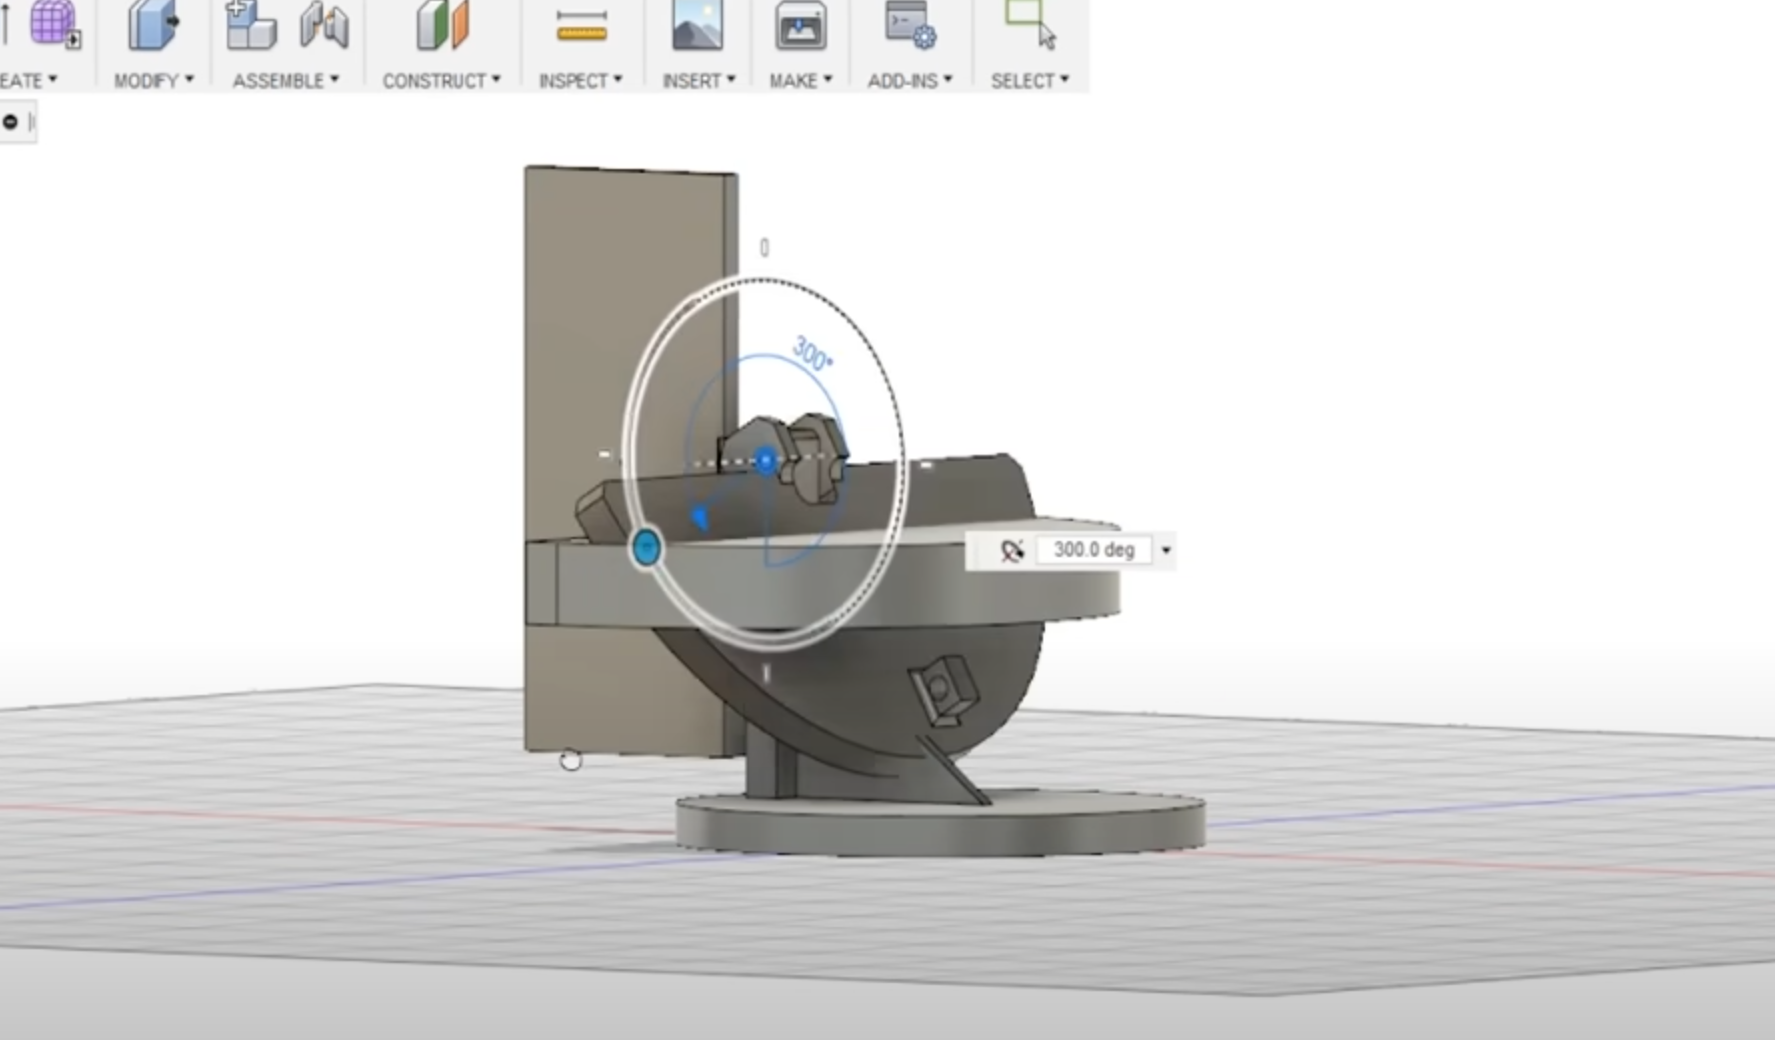
\includegraphics[width=\linewidth]{images/michael reeves.png}
    \caption{Digital twin of an animatronic doll rotating its jaw through 360 degrees}
    \label{fig:michaelreeves}
  \end{minipage}
\end{figure}

\subsection{Applications of Virtual Technology for Research}

VR being based on software means that all of the data being supplied to and received from the headset and peripherals can be tracked. This data can be used to study exactly how a person moves and reacts in a given scenario. \cite{baldominos2015approach}

During the filming of a music video for a concert to be in held in the video game Roblox, \cite{Roblox}, the members of the band 21 Pilots wore motion capture (mocap) suits to record their movements. The data from the mocap suits was used to animate the band members' characters in the game. \cite{YouTubeVideo21Pilots} In a comedic example of the movement data which can be captured, one of the band members, Josh, is seen in the software using a lavatory \cite{RedditPost21Pilots} as seen in figure \ref{fig:joshmocapconcert}.

\begin{figure}[h]
  \centering
  \begin{minipage}[b]{0.7\linewidth}
    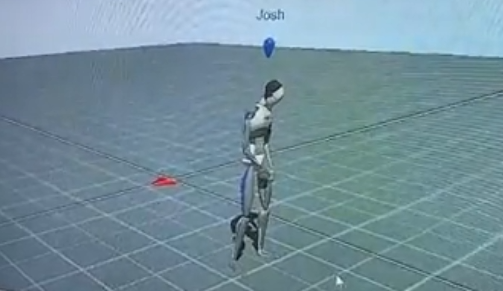
\includegraphics[width=\linewidth]{images/josh-mocap-concert.png}
    \caption{Josh from 21 Pilots using a lavatory in a mocap suit}
    \label{fig:joshmocapconcert}
  \end{minipage}
\end{figure}

Studying a person's eye movements can also be an effective way of measuring their competency or mental state in a given task. For example, people tend to fixate their gaze on a certain point when under extreme stress (sometimes known as tunnel vision) \cite{herten2017role}. Eye tracking is possibility in virtual reality \cite{clay2019eye} so could be used as a partial measure to measure a person's stress levels. 


\subsection{Creating Realistic Virtual Environments}

\subsubsection{Key Design Princples}

\subsubsection{Defining Realism}

- Research paper here about defining realism -

\subsubsection{Generation of HDRI Backdrops}

A HDRI backdrop can be used to 

\begin{figure}[h]
  \centering
  \begin{minipage}[b]{0.7\linewidth}
    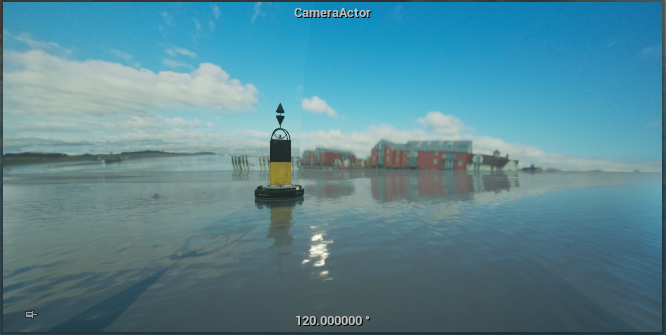
\includegraphics[width=\linewidth]{images/wivenhoe-buoy.png}
    \caption{A 3D scene next to The Jetty in Wivenhoe, Essex, UK with a buoy in the foreground}
    \label{fig:wivenhoeBuoy}
  \end{minipage}
\end{figure}

\begin{figure}[h]
  \centering
  \begin{minipage}[b]{0.7\linewidth}
    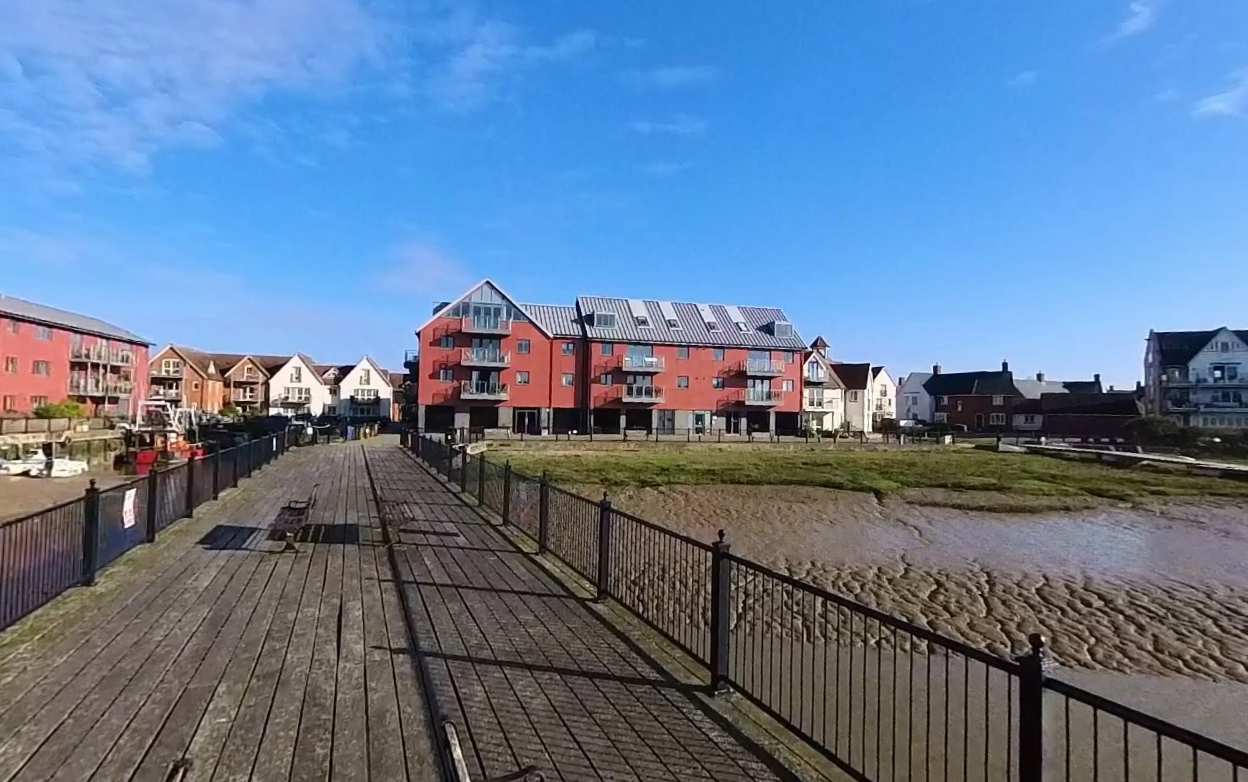
\includegraphics[width=\linewidth]{images/wivenhoe-google-maps.png}
    \caption{The same location as in figure \ref{fig:wivenhoeBuoy} in Google Maps. Image courtesy of Petrus Swart}
    \label{fig:wivenhoeGoogleMaps}
  \end{minipage}
\end{figure}

\subsubsection{Structure from Motion Photogrammetry} \label{sec:sfm}

Structure from Motion Photogrammetry (SfM) is a technique in which photographs can be used to created 3D models of objects or environments. These 3D models can then be used in virtual environments or 3D printed for further study. The results of photogrammetry can be comparable to those of Light Detection and Ranging (LiDAR) scanning and is very accessible, being achieve with a mobile phone camera and computer. \cite{iglhaut2019structure}

\begin{figure}[h]
  \centering
  \begin{minipage}[b]{0.7\linewidth}
    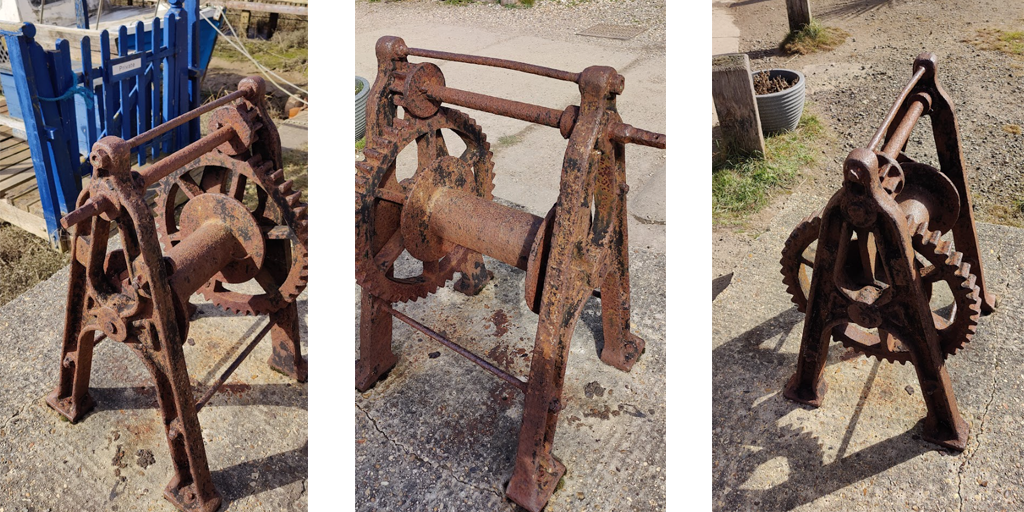
\includegraphics[width=\linewidth]{images/winch photogrammetry.png}
    \caption{Pictures taken of a winch located in Wivenhoe, Essex, UK}
    \label{fig:winchPhotogrammetry}
  \end{minipage}
\end{figure}

\begin{figure}[h]
  \centering
  \begin{minipage}[b]{0.7\linewidth}
    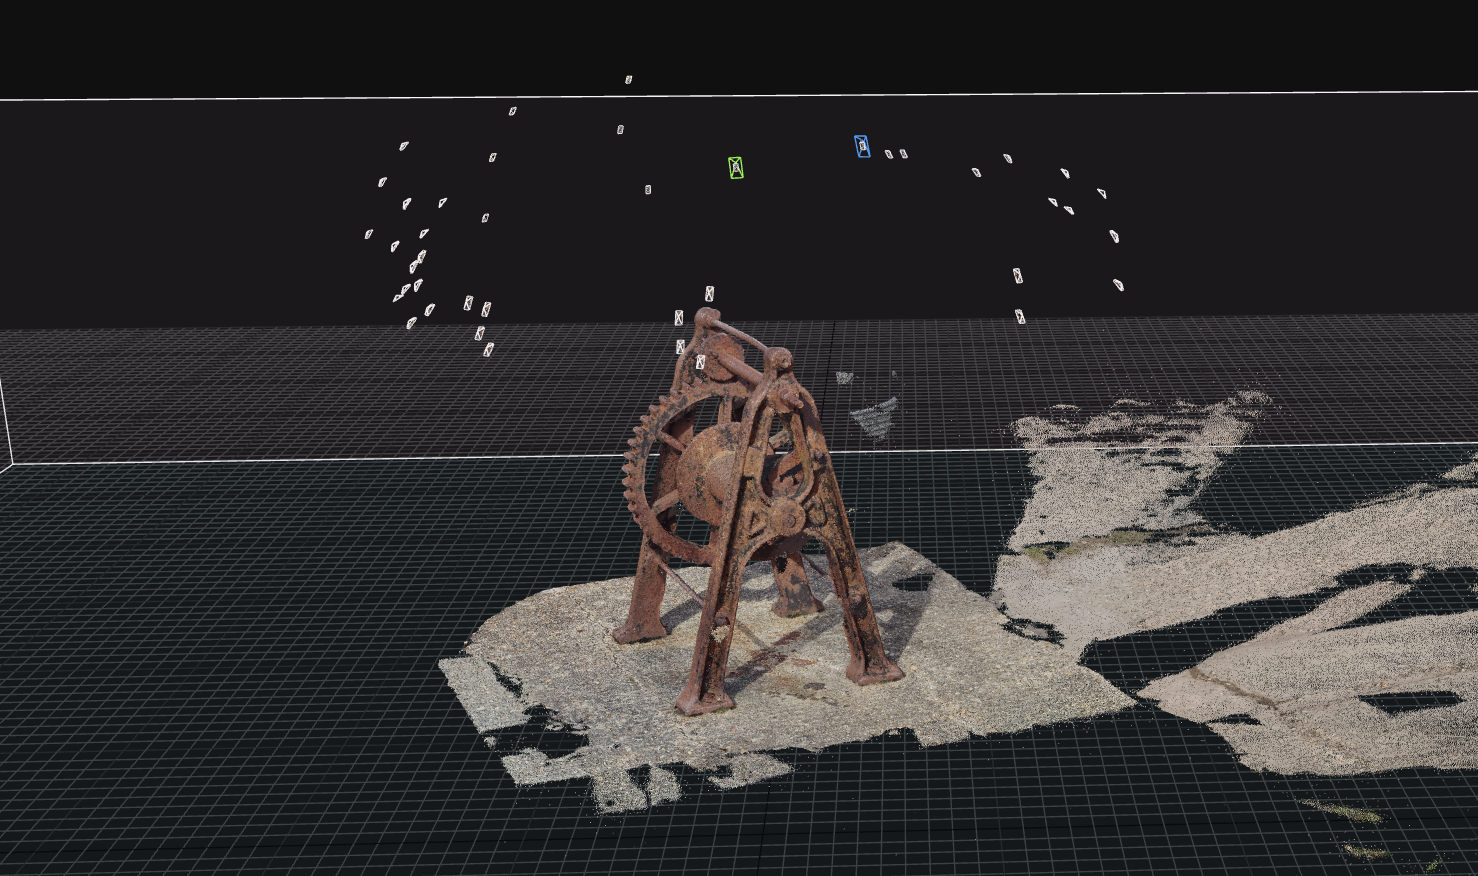
\includegraphics[width=\linewidth]{images/winch photogrammetry project.png}
    \caption{The results of SfM photogrammetry of a winch in Wivenhoe, Essex, UK}
    \label{fig:winchPhotogrammetryProject}
  \end{minipage}
\end{figure}

\subsubsection{3D Printing} \label{sec:3dprinting}

These results were achieved with a Flashforge 5M Adventurer Pro \cite{FlashForgeAdventurer5MPro} 3D printer using PLA, with a nozzle size of 0.4mm and a layer height of 0.2mm. The print time was approximately 1 hour and 50 minutes, using automatically generated tree supports.

\begin{figure}[h]
  \centering
  \begin{minipage}[b]{0.7\linewidth}
    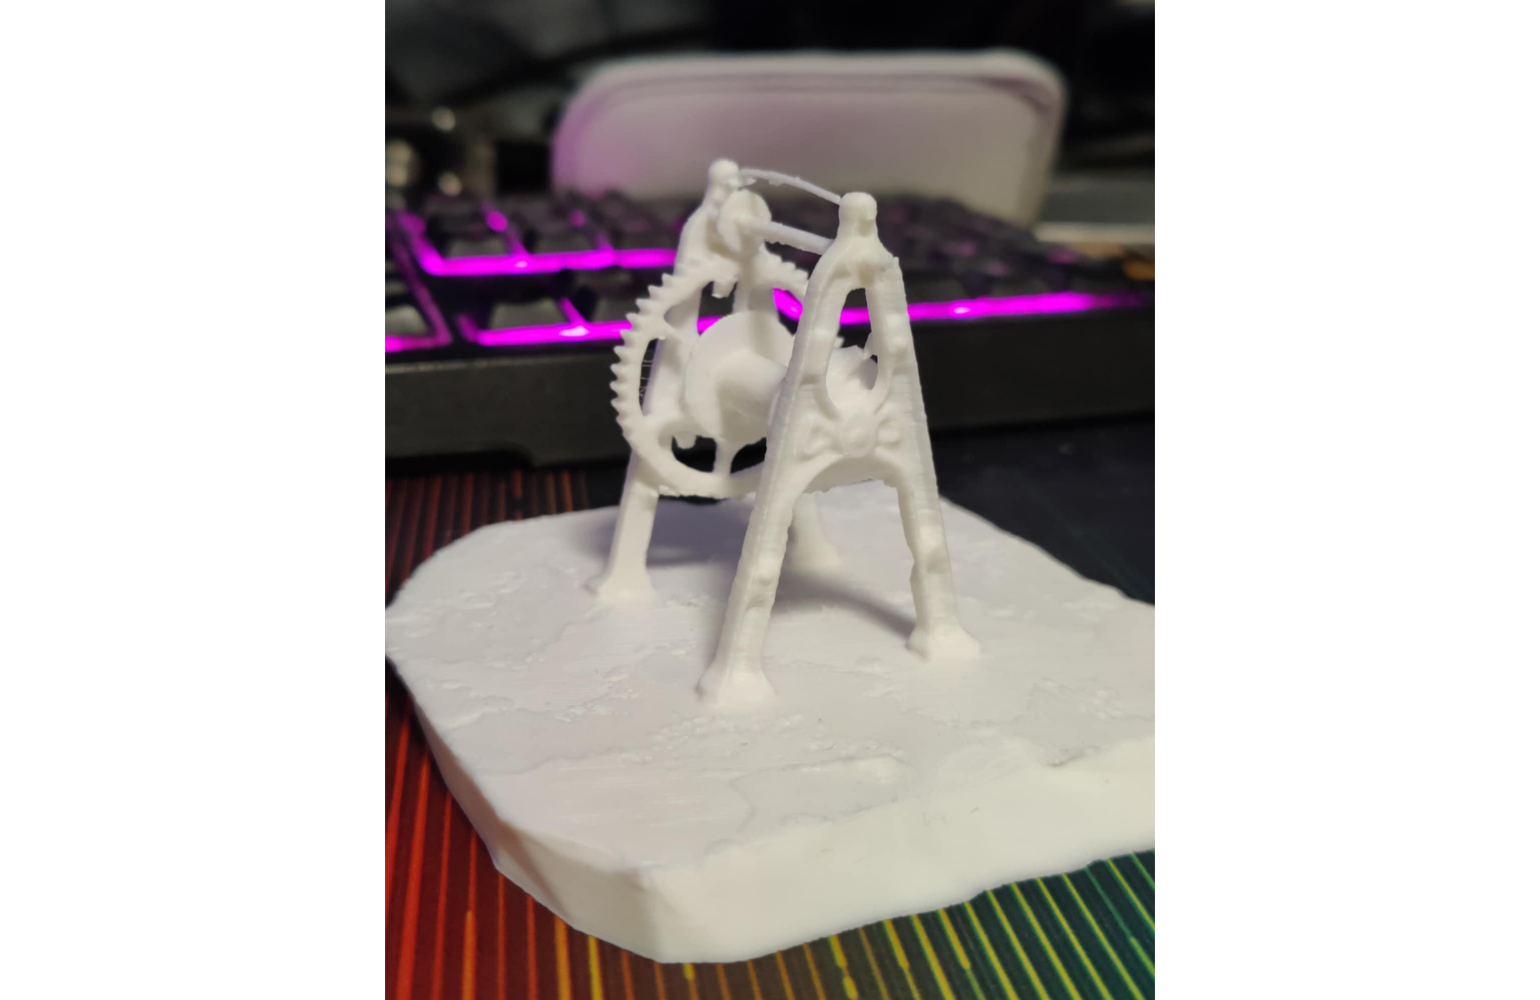
\includegraphics[width=\linewidth]{images/winch 3d model.png}
    \caption{A 3D printed model of the Wivenhoe winch as seen in figure \ref{fig:winchPhotogrammetryProject}}
    \label{fig:winch3dmodel}
  \end{minipage}
\end{figure}

\subsubsection{Tactile Models to Support Training in Virtual Environments}

These models can be made with a mix of Sfm photogrammetry \ref{sec:sfm} and 3D printing \ref{sec:3dprinting}.

\subsection{Measuring Stress Levels}

Data regarding the stress level of a participant can be attained by measuring a person's heart rate, heart rate recovery time, salivary cortisol and amylase. Further surveys and interviews can be conducted with volunteers to gather information. \cite{liu2018impact}

Eye-tracking solutions may also be used to measure stress levels in the same way as they have been used to measure competency in martitime navigation training. \cite{atik2019use}

% Perceived stress scale

% Galvanic skin response

Tried with myself and it worked after settling down for a while

Tried with Jasmine and could not get a reading, figured fingers might be too small

% Blink detection



\subsection{Application of Virtual Environments in Training for High-pressure Scenarios} \label{sec:applicationsOfVirtualEnvironments}

Training for high-pressure scenarios can be expensive and dangerous. From 1st January 2000 to 29th February 2024, 162 UK armed forces personnel died whilst on training or exercise. \cite{ukmod2024} In a report published by the UK Ministry of Defence, the cost of 105mm artillery shells between the commencement of Operation Herrick 17 and 17th December 2014 ranged from ~£50.00 to ~£2,812.00 per shell, depending on the type of shell and other factors. \cite{ukmod2015} Assuming a cost of £50.00 per shell (at the lower end of the scale), the cost of a battery of 6 guns firing 6 shells each, per fire mission, would be £1,800.00. This is a significant cost for a single training exercise which could potentially last weeks or more. Now scale this up to the cost of a year's worth of training for the entire UK armed forces and the cost becomes astronomical. For example, exercise Steadfast Defender involved ~90,000 troops and personnel, 50+ naval assets, 80+ air platforms and over 1,1000 combat vehicles. \cite{steadfastdefender24}

In 2024, an Apache helicopter deployed on an exercise in Jordan with the Utah National Guard crashed. \cite{intergalactic2024} No one was killed in the crash but the cost of the aircraft, as of the date of the crash, was around 50 million USD. \cite{cbsaustin2024} It is theorised that the crash was caused by an experiened jet pilot attempting to control the rotary wing aircraft and causing an irrecoverable stall. \cite{carlisle2024}

On the 13th of January, 2024, the 47th Separate Mechanized Brigade of the Ukrainian Army reported the destruction of a Russian T-90 Proryv tank. \cite{malyasov2024} It has been proven that the T-90's external systems (such as optics) were destroyed by the main cannon of a Bradley AFV, commanded by Serhiy of the Ukrainian Army. In an interview with Serhiy, he stated that he knew which parts of the tank to fire at (to damage the external systems) as he had practised in "video games" \cite{militaryconflict2025} (it is likely, although unconfirmed, that he is referring to War Thunder \cite{warthunder}).

University students can undertake courses in maritime operations and technology, such as the one offered by the University of South Eastern Norway. They can use a ship bridge simulator to practice their skills in a controlled environment as seen in Figure \ref{fig:maxvdhnorway}.

\begin{figure}[h]
  \centering
  \begin{minipage}[b]{0.9\linewidth}
    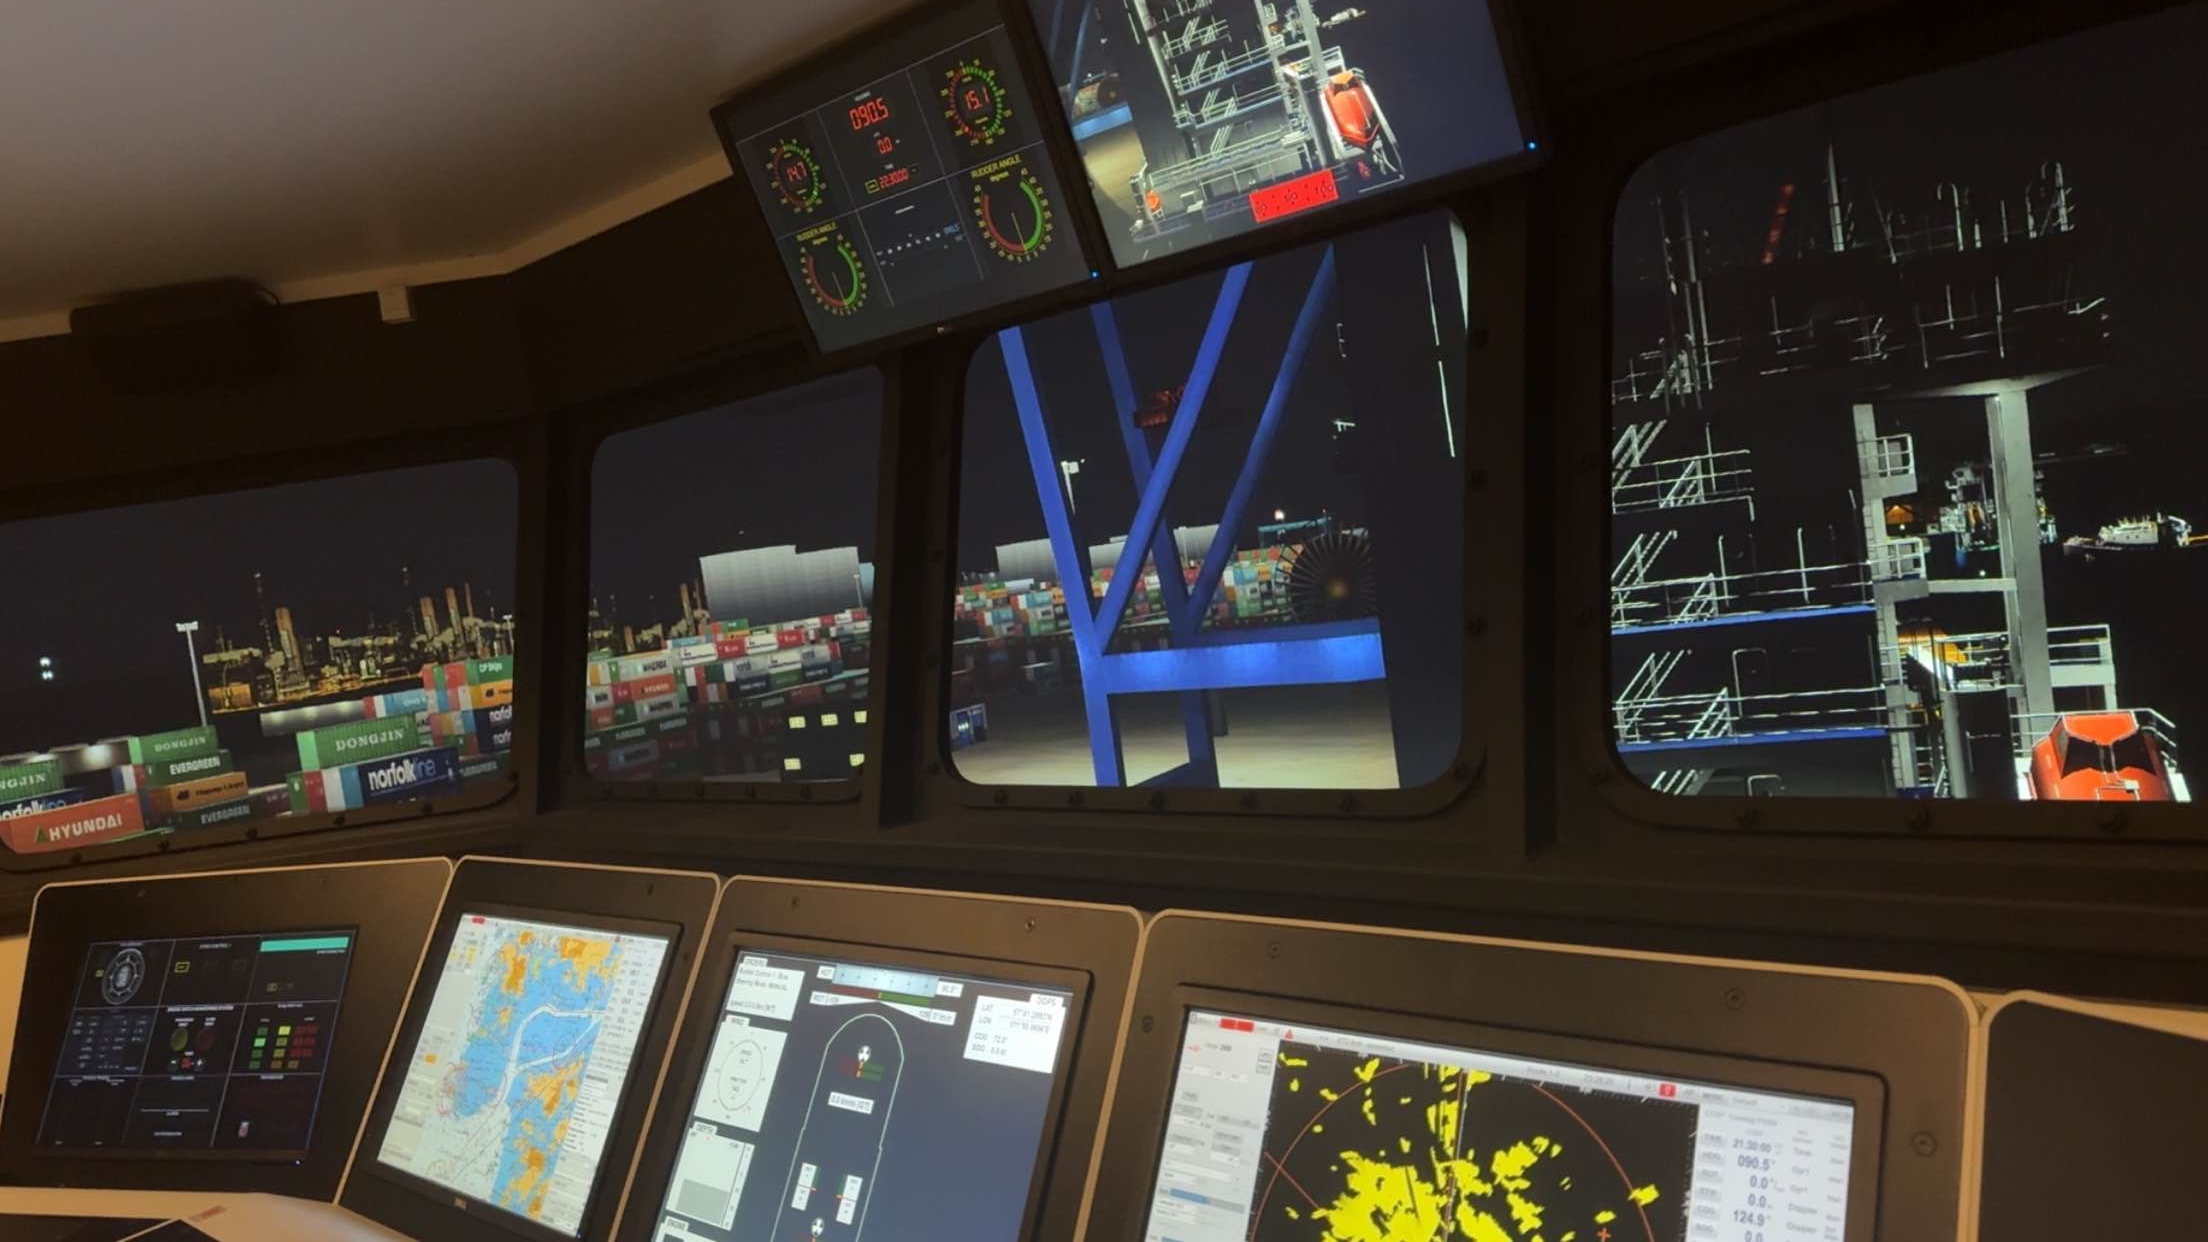
\includegraphics[width=\linewidth]{images/max_vdh_norway.jpg}
    \caption{A simulated ship bridge simulator, with screens and physical controls, at the University of South Eastern Norway courtesy of Max Van Der Haagen, student.}
    \label{fig:maxvdhnorway}
  \end{minipage}
\end{figure}

\subsection{Challenges with Maritime Experimentation}

% https://journals.plos.org/plosone/article/file?id=10.1371/journal.pone.0186871&type=printable

\subsubsection{Gathering Data}

Ensuring accuracy and reliability

\subsubsection{Minimising Risk}

\subsubsection{Logistics}

\subsubsection{Ethical Considerations}



\subsection{Preparation for Experiments in Potentially Dangerous Situations}

\subsubsection{Gathering Data}

Privacy Concerns

\subsubsection{Minimising Risk}

Ensuring people are comfortable with water and understanding how to stay safe in water

Intake questionairres 

Apparatus

\subsection{Preparation for Maritime Experimentation}

\subsubsection{Volunteers}

Intake questionairres can be used to understand the knowledge and/or experience a volunteer may have before starting an experiment. For example, people with a background in playing video games may be more likely to have experienced or have an understanding of virtual reality before the experiment begins. 

Eye relief plays a huge part in the perceived fidelity of a virtual environment and an inexperienced user of virtual reality might not realised that the view being blurry is not intended. As with other forms of optics which use light refraction to produce an image, factors such as field of view, freedom from glare, alignment, freedom from fogging \cite{angel2005examination} are concerns which inexperienced users might not know how to address. They are also very difficult for the researcher to adjust for the volunteer as they can't see what the volunteer can see.

\subsubsection{Apparatus}

Apparatus

\subsection{Performance Measures} \label{performanceMeasures}

https://www.taylorfrancis.com/chapters/edit/10.4324/9781315243092-21/performance-measurement-simulation-based-training-eduardo-salas-michael-rosen-janet-held-johnny-weissmuller

Mutual performance monitoring can be used in conjunction with questionairres to measure the performance of volunteers in a given scenario. \cite{salas2017performance} Peer reviews can offer insite into how a person is performing in a given scenario and potentially cover areas which data-driven metrics might not have caught. Furthermore, peer reviews can be used to identify results which may have been misinterpreted from data. 

\subsubsection{Simulation}

\subsubsection{Real-world}

\subsection{Preparation for Simulator Experimentation}

\subsubsection{Volunteers}

Selection and Training of Participants

\subsubsection{Apparatus}

\subsection{Consumer-ready Simulation Software}

\subsection{Data Collection}

\subsubsection{Simulation}

In a simulation, the data is produced by the software so is normally accessible and therefore easy to collect. For example, the consumer ready simulation software Arma 3 provides a scripting language inside it which can be utilised by server managers to track what happens in an event. One such piece of software, Operation Capture and Playback 2 (OCAP) allows for people to watch back a 2D representation of their game for recreation and performance analysis as discussed in section \ref{sec:performanceMeasures}.

\subsubsection{Real-world}

\section{Building Virtual Environments for Training in Unreal Engine 5}

\subsection{Introduction}

\subsection{Digital Twins}

\subsection{Unreal Engine 5}

\section{Human Perception and Differentiation of Real and Virtual Environments}

\subsection{Introduction}

\subsection{Methodology}

\subsection{Experiment 1 - Mutilus}

\subsubsection{What is Mutilus?}

\subsubsection{Prototype Experiments}



\subsubsection{Results}

\section{Applications of this Research}

In my experience, consumer-ready software is often brushed aside in favour of the "official" version, with seemingly little effort put into determine whether the consumer-ready version would suffice for the task. One such example is the prevalence of software such as Microsoft Teams \cite{MicrosoftTeams} and Zoom \cite{Zoom} being used by small businesses instead of free software such as Discord \cite{Discord}. Discord provides the functionality, which everyone has grown to expect from software such as Zoom, such as large voice calls, instant messaging and screen-sharing without the security risks which Zoom was (and still is) infamous for, especially during the COVID-19 pandemic. On top of that, Discord is free. 

This is also true in the world of simulators for training purposes. Using software such as Virtual Battlespace for training is considered the norm in military training with the consumer-ready version Arma appearing to provide sufficient features for training, at a fraction of the price. 

This research could help give small businesses and organisations more confidence to try out consumer-ready training software for their training needed. 



\subsection{Training for Stressful Scenarios}

\section{Machine Learning to Assess Performance in Maritime Navigation}

% Make a model which spots objects in the scene and then uses that to determine how well a person is performing in a maritime navigation scenario. This could be useful for randomly generated scenarios where the user has to find a specific object in the scene, such as a buoy or a ship and not having supervisors there to monitor the user. This could also be used in screen recording. Ultimately, Unreal Engine 5 could be used to identify the locations internally but what if the user is using a different piece of software because a PC can't run it? Inference is generally less resource intensive than training so a model could be trained in Unreal Engine 5 on a good PC and then tested on a laptop with a less powerful GPU.

% The justification here is also that, yes, Unreal Engine 5 is all knowing about its environments. However, understand the world from the user's view point is crucial for effective training and assessment. A comparison of the reality of the environment to the user's performance could be unfair as, for example, simulated foggy weather could hinder performance whereas data from Unreal Engine 5 could indicated that the user should have been able to see the object they were looking for.

\section{Automated Generation of Labelled Synthetic Data for Machine Learning}

\subsection{Introduction}



\subsection{Methodology}

\subsubsection{Understanding the Data Needed}

\subsubsection{Objects of Interest}

\subsubsection{Environments}

\subsubsection{Taking Pictures}

% Talk about the difference in Arma 3 and Unreal Engine 5. With Arma 3, you can run a script which can sleep so the camera positioning was easy to achieve. However, Unreal Engine executes the code per frame so the camera positioning was more difficult to achieve.

\subsubsection{Labels}

\subsection{Results}

\section{Methodology}

\subsection{Simulation Variables and Physiological Stress}

When playing online competitive games that involve controlling a character in a simulated dangerous environment, players often report feelings of stress. Whether it's the end of a round in Counter-Strike, hiding from enemy players in Arma, or speaking to a simulated ghost in Phasmophobia, these scenarios tend to evoke a stress response, even though there is no real danger to the player themselves.

Understanding exactly what it is about these scenarios that triggers a stress response could be useful in preparing individuals for real-life high-stress situations, such as those faced by police officers, military personnel, and maritime professionals.

\subsection{Experiment Design}

\subsubsection{Fractional Factorial Design}



\subsubsection{Simulation Variables}

\subsubsection{Physiological Stress Indicators}

\subsection{Data Collection}

\subsubsection{Physiological Data}

\subsubsection{Simulation Data}

\subsection{Data Analysis}

\subsubsection{Statistical Analysis}

\subsubsection{Machine Learning}

\section{Results}

\section{Discussion}

\section{Conclusion}

\section{References}

\bibliographystyle{ieeetrans}
\bibliography{references}

\section{Appendices}



\end{document}
